\documentclass[10.5pt,a4paper]{article}
% Ortak onbilgi: uc "Study of Simulation Tools" raporu icin. Derleme: tectonic -X compile <dosya>.tex (rapor\ klasorunde)
\usepackage{fontspec}
\setmainfont{georgia}[Path=../fontlar/,Extension=.ttf,BoldFont=georgiab,ItalicFont=georgiai,BoldItalicFont=georgiaz]
\setsansfont{arial}[Path=../fontlar/,Extension=.ttf,BoldFont=arialbd,ItalicFont=ariali,BoldItalicFont=arialbi]
\setmonofont{consola}[Path=../fontlar/,Extension=.ttf,BoldFont=consolab,ItalicFont=consolai,BoldItalicFont=consolaz,Scale=0.86]
\usepackage[a4paper,left=2.2cm,right=2.2cm,top=1.9cm,bottom=1.8cm]{geometry}
\usepackage{xcolor,graphicx,titlesec,enumitem,amsmath,booktabs,xltabular,listings,fancyhdr,caption}
\emergencystretch=3em
\definecolor{ink}{HTML}{1F2937}\definecolor{acc}{HTML}{1D4ED8}\definecolor{muted}{HTML}{6B7280}\definecolor{codebg}{HTML}{F3F4F6}
\color{ink}
\titleformat{\section}{\sffamily\bfseries\large\color{acc}}{}{0pt}{}
\titlespacing*{\section}{0pt}{9pt}{3pt}
\titleformat{\subsection}{\sffamily\bfseries\normalsize}{}{0pt}{}
\titlespacing*{\subsection}{0pt}{6pt}{2pt}
\setlength{\parindent}{0pt}\setlength{\parskip}{4pt plus 1pt}
\setlist{itemsep=1pt,topsep=2pt,parsep=0pt}
\pagestyle{fancy}\fancyhf{}\renewcommand{\headrulewidth}{0.3pt}
\fancyhead[L]{\sffamily\footnotesize\color{muted} EHB415 \textbullet\ Study of Simulation Tools}
\fancyfoot[C]{\sffamily\footnotesize\color{muted}\thepage}
\captionsetup{font={sf,footnotesize},labelfont=bf,labelsep=period,skip=2pt}
\lstset{basicstyle=\ttfamily\footnotesize,backgroundcolor=\color{codebg},frame=single,rulecolor=\color{codebg!70!black},
  breaklines=true,columns=fullflexible,keepspaces=true,showstringspaces=false,aboveskip=4pt,belowskip=6pt,
  literate={ğ}{g}1 {ş}{s}1 {ı}{i}1 {ü}{u}1 {ö}{o}1 {ç}{c}1}
\newcommand{\baslik}[2]{%
  {\sffamily\color{muted}\small EHB415 Dönem Projesi \textbullet\ 2026--2027 Güz\par}
  {\sffamily\bfseries\Large Study of Simulation Tools: #1\par}
  {\sffamily\small #2\par}
  \vspace{-2pt}{\color{acc!40}\rule{\textwidth}{0.8pt}}\par}
\IfFileExists{isimler.tex}{\input{isimler}}{\newcommand{\taha}{[Ad Soyad -- No]}\newcommand{\aziz}{[Ad Soyad -- No]}\newcommand{\fatih}{[Ad Soyad -- No]}\newcommand{\nihat}{[Ad Soyad -- No]}}

\begin{document}
\baslik{OCUDU}{Hazırlayan: \fatih}

\section*{1. Projedeki yeri ve araç seçimi}
OCUDU, srsRAN Project'in devamı olan ve Linux Foundation çatısı altında geliştirilen açık kaynaklı bir \textbf{gerçek 5G baz istasyonu (gNB) yazılımıdır}. ns-3 gibi bir model değil, gerçek protokol kodudur. Projemizde, sensing için ayrılan kaynağın (PRS) haberleşmeye maliyetini gerçek bir zamanlayıcı (scheduler) üzerinde ölçmek için kullanılacak; bu, ns-3 sonuçlarına güvenilirlik katar. Gerçek bir radyo (USRP) gerekmeden çalışabilmesi için ZeroMQ (sanal RF) ve \texttt{testmode} özellikleri kullanıldı.

\section*{2. Kurulum}
\begin{center}\sffamily\small
\begin{tabular}{@{}ll@{}}
\toprule
Ortam & Windows 11 üzerinde WSL2, Ubuntu 24.04.5 LTS \\
Derleyici ve araçlar & Clang 18.1.3, CMake 3.28.3, ccache \\
Yazılım sürümü & OCUDU \texttt{release\_26\_10}, 26.10.0 (commit e0db566) \\
Seçenekler & \texttt{ENABLE\_ZEROMQ=ON}, \texttt{ENABLE\_EXPORT=ON}; yalnızca \texttt{gnb} hedefi \\
Süre ve disk & yaklaşık 23 dakika (\texttt{-j4}), yaklaşık 0,6 GB \\
\bottomrule
\end{tabular}
\end{center}
Resmi kurulum sayfası gcc 15.2 veya üstünü ya da Clang 14 ve üstünü önerir. Ubuntu 24.04'te gcc 13.3 olduğu için \textbf{Clang 18} kullandık. Komutlar (ayrıntı: \texttt{kurulum/05-ocudu.md}):
\begin{lstlisting}
sudo apt-get update
sudo apt-get install -y cmake make gcc g++ clang pkg-config \
    libmbedtls-dev libsctp-dev libyaml-cpp-dev libgtest-dev \
    libfftw3-dev libeigen3-dev libzmq3-dev ccache
mkdir -p ~/ehb415 && cd ~/ehb415
git clone --depth 1 --branch release_26_10 https://gitlab.com/ocudu/ocudu.git
cd ocudu && mkdir -p build && cd build
CC=clang CXX=clang++ cmake ../ -DENABLE_EXPORT=ON -DENABLE_ZEROMQ=ON \
    -DCMAKE_C_COMPILER_LAUNCHER=ccache -DCMAKE_CXX_COMPILER_LAUNCHER=ccache
make -j4 gnb
\end{lstlisting}
CMake çıktısında \texttt{The CXX compiler identification is Clang 18.1.3} ve \texttt{Found libZEROMQ} satırları görünmelidir.

\section*{3. Karşılaşılan sorunlar ve çözümleri}
\begingroup\sffamily\small
\begin{xltabular}{\textwidth}{@{}p{4.3cm}X@{}}
\toprule
\textbf{Sorun} & \textbf{Neden ve çözüm} \\
\midrule
CMake çıktısında \texttt{Found libZEROMQ} yok & ZeroMQ yalnızca yapılandırma sırasında algılanır. \texttt{libzmq3-dev} kurulup \texttt{build} klasörü silindi ve \texttt{cmake} yeniden çalıştırıldı. \\
Derleme çıktısında ``error'' kelimesi & Dosya adlarında geçiyor (\texttt{..\_error\_handler\_impl.cpp}). Gerçek hata \texttt{error:} ile ve dosya:satır bilgisiyle başlar. \\
\texttt{256QAM MCS table cannot be used for PDSCH with fallback DCI format} & İlk testmode denemesinde \texttt{pdsch/pusch mcs\_table: qam64} ayarı eksikti. Yapılandırma dosyasına eklenince hücre açıldı. \\
\texttt{Scheduling priority of thread ... not changed. Not enough privileges} & Gerçek zamanlı öncelik için \texttt{sudo} gerekir. WSL'de zararsızdır, hücrenin açılmasını engellemedi. \\
Günlükte \texttt{Real-time failure in RU: received late DL request} & WSL2 çekirdeği gerçek zamanlı olmadığı için beklenen bir uyarıdır. \\
Ölçüm tablosu görünmüyor & Tablo yalnızca etkileşimli terminalde (TTY) görünür. Program çalışırken \texttt{t} yazıp Enter'a basmak gerekir. \\
\bottomrule
\end{xltabular}
\endgroup

\section*{4. Örnek çalıştırma}
Kurulumu doğrulamak için gNB'yi radyo ve çekirdek ağ olmadan çalıştırdım (\texttt{ru\_dummy}, \texttt{no\_core}, 1 sanal kullanıcı; yapılandırma: \texttt{ocudu\_testmode.yml}). Program başladıktan sonra \texttt{t} yazıp Enter'a basarak canlı ölçüm tablosunu açtım.
\begin{lstlisting}
cd ~/ehb415/ocudu/build/apps/gnb
./gnb --version
./gnb -c ~/ehb415/ocudu_testmode.yml
\end{lstlisting}
\begin{figure}[h!]
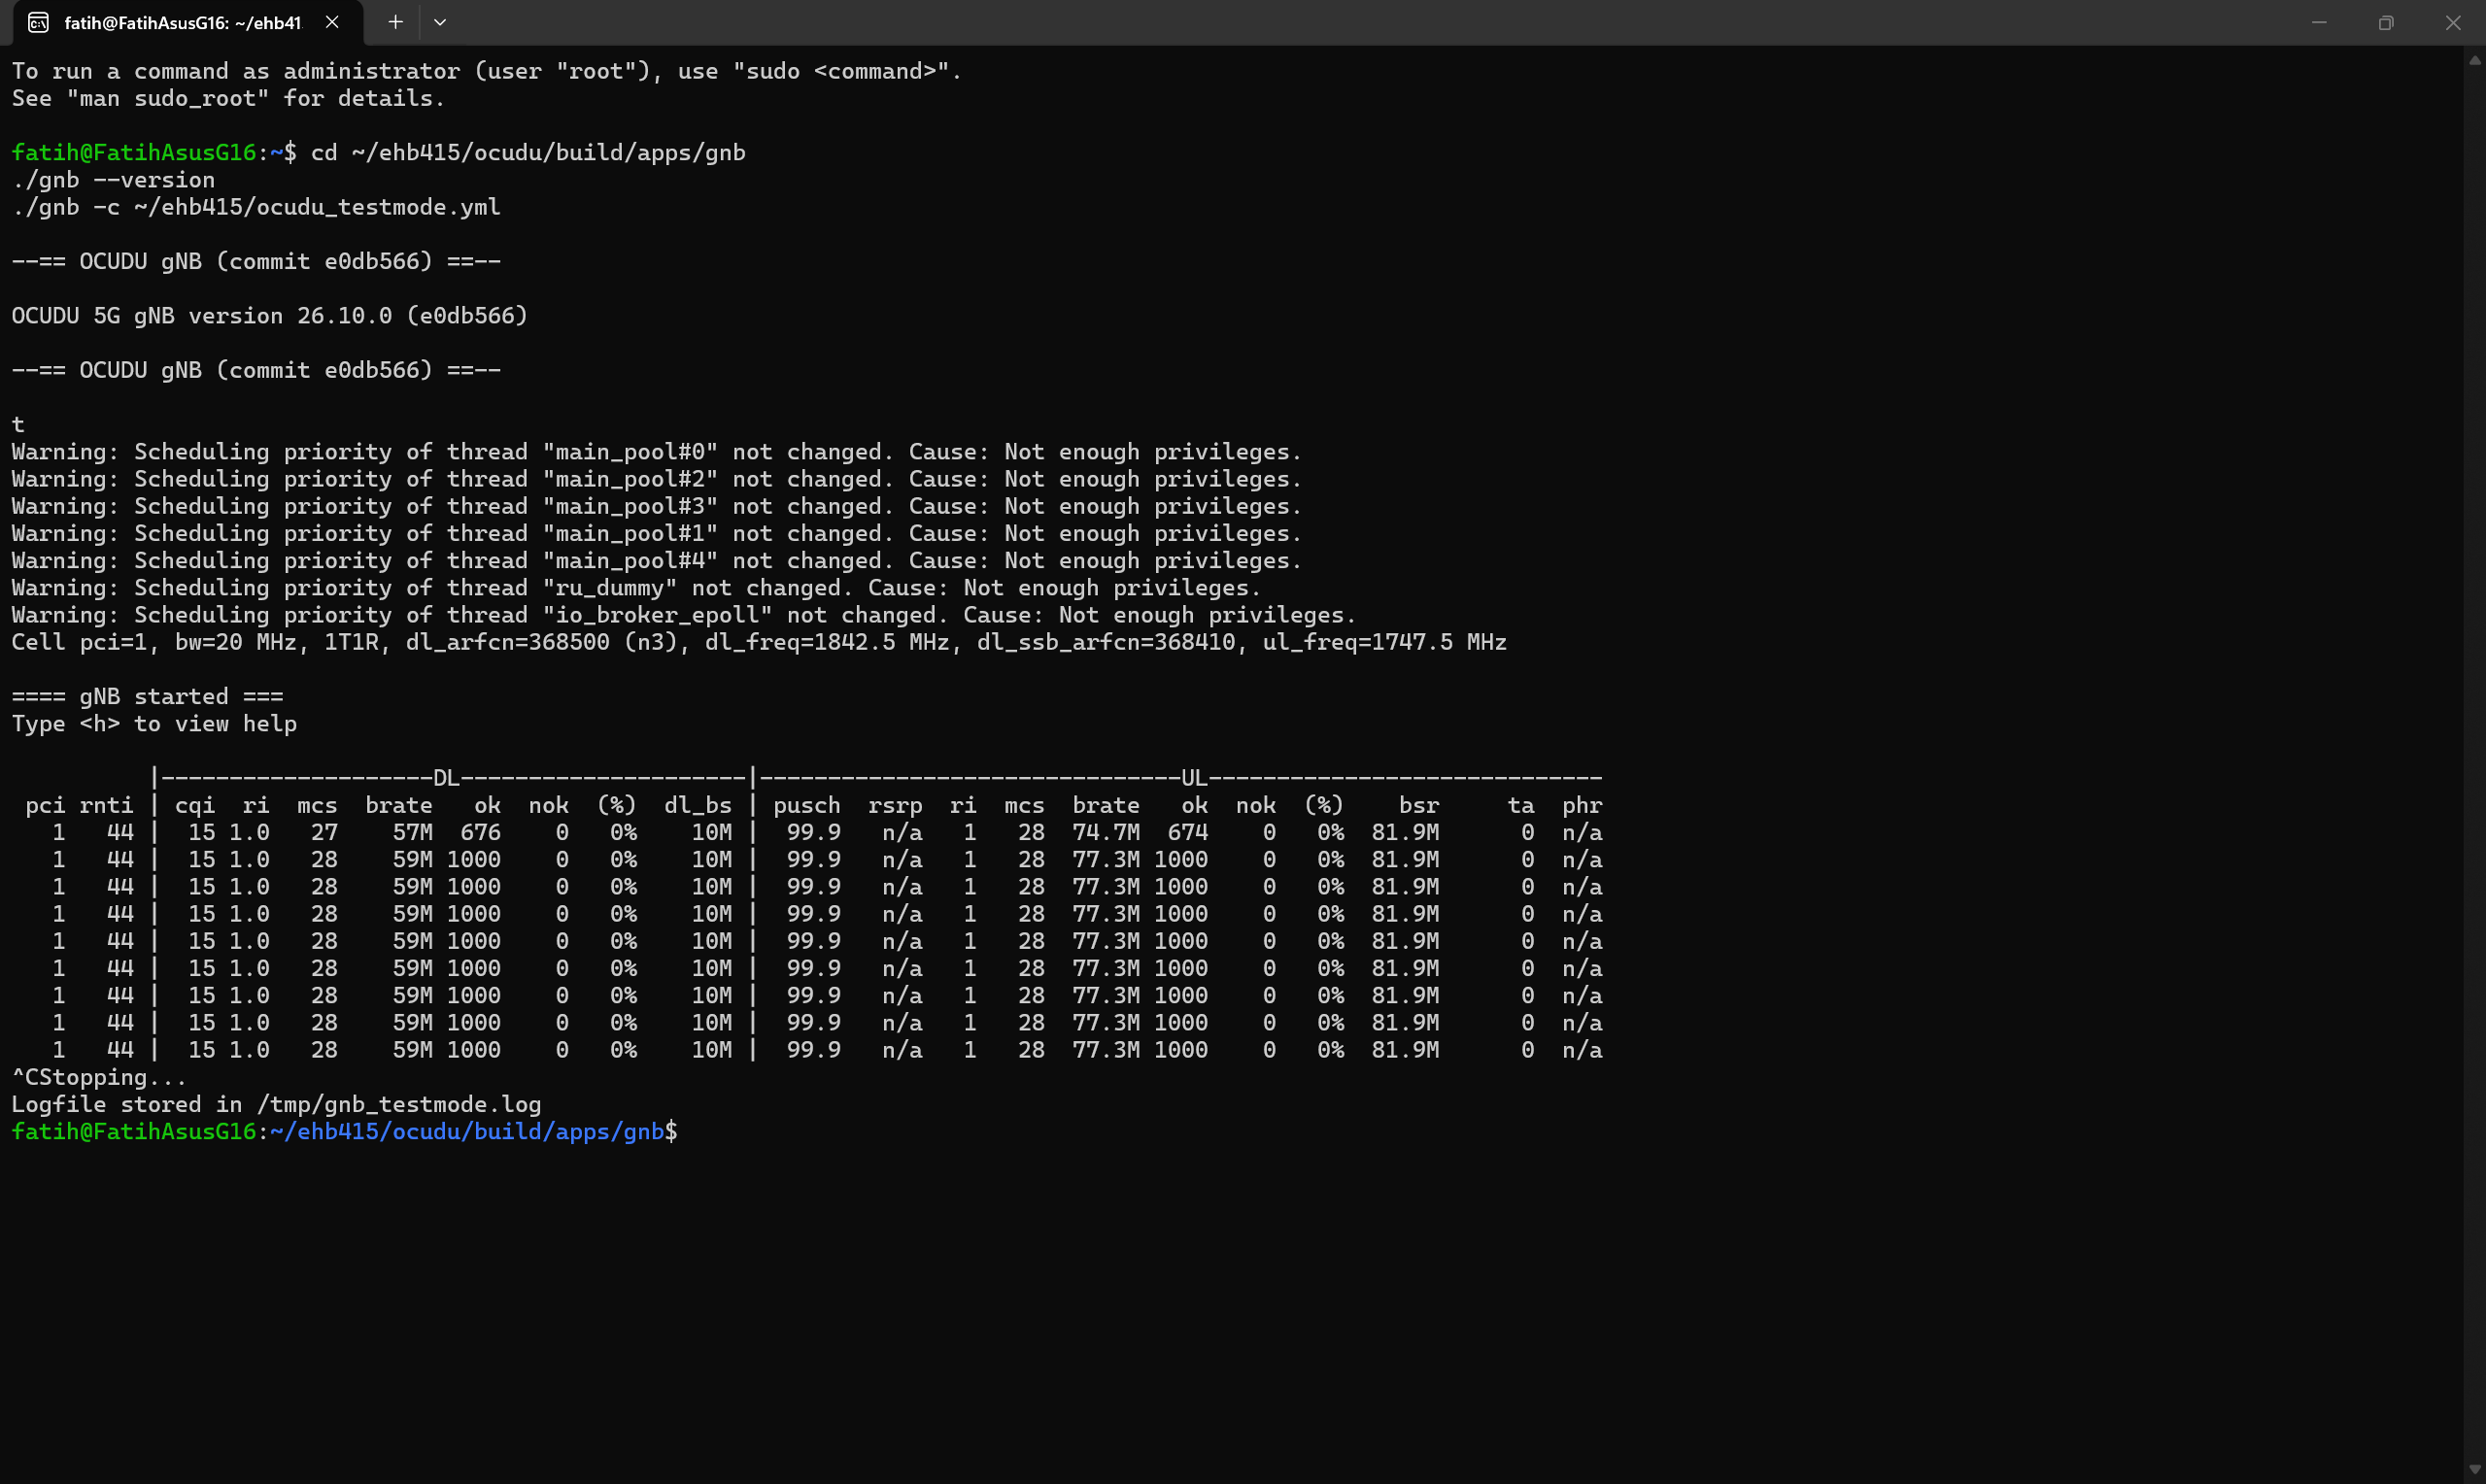
\includegraphics[width=\textwidth]{img/ocudu_terminal.png}
\caption{\texttt{gnb --version}, hücrenin açılması ve canlı ölçüm tablosu (WSL2 Ubuntu).}
\end{figure}
Çıktıda 26.10.0 (e0db566) sürümü ve n3 bandında 20\,MHz, 1T1R bir hücrenin açıldığı görülüyor. Tablonun kararlı satırlarında \textbf{DL hızı yaklaşık 59 Mbps, UL hızı 77,3 Mbps} ve her iki yönde başarılı blok sayısı \textbf{1000 blok/s} okundu. Ctrl+C'den sonra program \texttt{Stopping} mesajıyla düzgün kapandı. Bu çıktılar OCUDU'nun radyosuz test ortamında çalıştığını ve ölçüm üretebildiğini gösteriyor.

\section*{5. Değerlendirme ve sonraki adımlar}
OCUDU 26.10.0 derlendi ve testmode'da çalıştı. Sınırlamalar: (i) srsUE ve Open5GS ile uçtan uca test \textbf{yapılmadı}; resmi dokümandan aktarıldı, bu kurulumda çalıştırılmadı. (ii) WSL2 gerçek zamanlı olmadığından gerçek radyo (USRP) bağlantısı desteklenmiyor; bu proje için gerekmiyor. Sonraki adımlar:
\begin{itemize}
\item PRS (konumlama referans sinyali) periyodunu değiştirip DL hızındaki düşüşü ölçmek (PRS yokken 59,0 Mbps).
\item Birden fazla sanal kullanıcıyla aynı deneyi tekrarlamak.
\item Açık soru: 4 sembollük PRS neden 12 sembollük PRS ile aynı kaybı veriyor? Zamanlayıcı kodunda (\texttt{intra\_slice\_scheduler.cpp}) PDSCH için hangi sembol aralığına bakıldığı incelenecek.
\end{itemize}
\end{document}
